\documentclass{standalone}
\usepackage{tikz}

\begin{document}

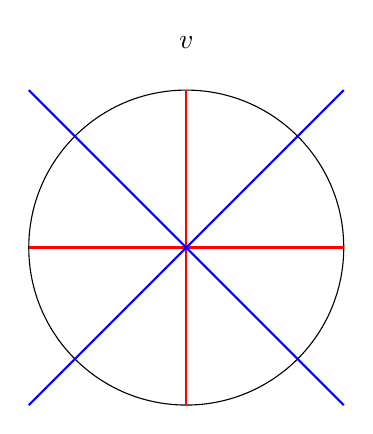
\begin{tikzpicture}[scale=2]

% Define coordinates for clarity
\def\x{0}
\def\y{0}
\def\r{1} % radius of the circle

% Draw the white circle
\draw[fill=white] (\x, \y) circle (\r);

% Draw the labels for the circle
\node at (\x, \y+\r+0.3) {$v$};

% Draw the red lines
\draw[red, thick] (\x-\r, \y) -- (\x+\r, \y); % horizontal line
\draw[red, thick] (\x, \y-\r) -- (\x, \y+\r); % vertical line

% Draw the blue lines
\draw[blue, thick] (\x-\r, \y-\r) -- (\x+\r, \y+\r); % diagonal line from bottom-left to top-right
\draw[blue, thick] (\x+\r, \y-\r) -- (\x-\r, \y+\r); % diagonal line from top-left to bottom-right

\end{tikzpicture}

\end{document}